\subsection{The scheme against neural networks}


1. Et kontrollert eksperiment (den viktigste).
Nøyaktig som du sier: ved å ta knekken ut av nettets oppgave skiller dere to mulige feilkilder:

er det knekken som gjør nettet dårlig?
eller er nettet dårlig til opsjonsproblemet generelt?



In Figure~\ref{fig:kink_decomp} our main takeaway is that a kink-free g does not change the scope of the project, just the form. From pointy to smooth is exactly what tanh-network can learn. The figure show why the naive net is going to fail. 

Our naive g is essentially the payoff diagram in the top (black dashed line). 

\begin{figure}[htbp]
\centering
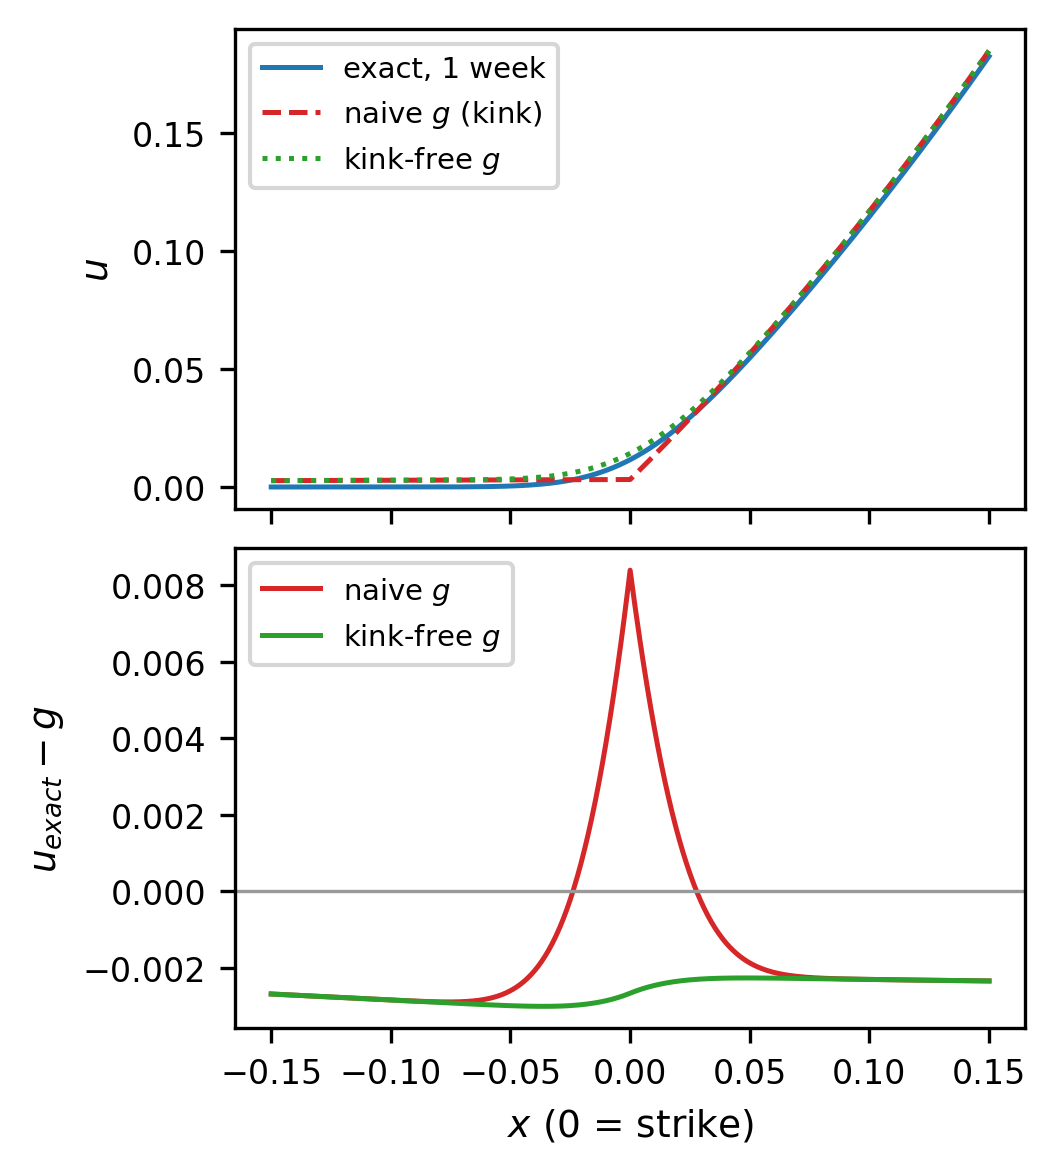
\includegraphics[width=\columnwidth]{Code/figures/kink_decomposition.png}
\caption{\textbf{Top panel:} The solution by 1 week,. \textbf{Bottom panel:} $u_{exact} - g$. For a naive g}
\label{fig:kink_decomp}
\end{figure}

    
